%%% Local Variables: 
%%% mode: latex
%%% TeX-master: "../KanjiHWR"
%%% End: 

\chapter{Technical Design of the Application}
\label{chap:technicaldesign}
%xxx untersuche dieses kapitel auf:
% die argumentationssequenz "folgende anforderungen, 
% folgende loesungsmoeglichkeiten,
% die gewaehlte loesungs entspricht den anforderungen am besten"
% NICHT: folgendes problem, erstbeste loesung, fertig
% stattdessen: zeige loesungsmoeglichkeiten

%xxx - Why this section? 
%xxx   The purpose of this section is 
%xxx   It would be off purpose, if 
%xxx - What goes into this section?
%xxx   The main content of this section is 
%xxx   * if describing a problem: why is the problem relevant.
%xxx   * if describing a solution to a problem: what alternatives were
%xxx     there to solve it, why was this solution chosen? 
%xxx     what made it the best choice? was it the optimal solution?
%xxx - How will this section be structured and organised?
%xxx   The organisational structure of the section 
%xxx - In what style will it be written?
%xxx   The style of writing will be 
%xxx - Next action - what to write first?
%xxx   The next part to write is



The focus of this chapter is on the general architectural choices made during
the development of the system. In this chapter, the technical design aspects 
of the application are described. The general system architecture is layed out in
section~\ref{sec:systemarchitecture}. It contains the global view on the software
architecture in section~\ref{sec:globalarchitecture}, the data flow in within
the system in section~\ref{sec:arch:systemdataflow} and describes the design
of the individual modules in section~\ref{sec:arch:softwaremodules}.
Section~\ref{sec:frameworkanddevices} describes the technical set-up and 
framework choices. However, the handwriting recognition engine is described 
in detail in a separate 
section~(see chapter~\ref{chap:handwritingrecognitionengine}).

\section{System Architecture}
\label{sec:systemarchitecture}

The system architecture of the Kanji Coach follows the requirements of an 
e-learning environment dealing with the specific difficulties for learners 
of the Japanese script (see chapter~\ref{chap:japanasescript}) and those of an 
on-line handwriting recognition. Techniques of handwriting recognition are 
reviewed in chapter~\ref{chap:onlinehwr}. The general requirements of an 
e-learning application are presented in chapter~\ref{chap:elearning}. 
The resulting specific conceptual design choices have been 
layed out in chapter~\ref{chap:conceptualdesignofkanjicoach}. This
section deals with the technical aspects of the system design.

\subsection{Global Architecture}
\label{sec:globalarchitecture}

The global architecture of the application follows the Model-View-Controller
(MVC) design pattern. This paradigm is used as a general model, however, 
it is not designed the strict way proposed by~\shortcite{Krasner1988}.
Figure~(\ref{fig:modelviewcontroller}) shows the general set-up of the 
MVC design pattern after~\shortcite{Krasner1988}. xxx: Also 
figure~(\ref{fig:modelviewcontroller2}) - decide how it should be done and use
the appropriate gfx. xxx!
In the MVC paradigm the \emph{model} is a domain-specific software, 
an implementation of the central structure of the system. It can be a simple
integer, representing a counter or it could be a higly complex object structure, 
even a whole software module. The \emph{view} represents anything graphical. 
It requests data from the model and displays the result. The \emph{controller} 
is the interface between the model and the view. It controls and scheduls the 
interaction between the input devices, the model and the 
view~\shortcite{Krasner1988}.
%xxx Make this a graphic, not a photographic image of a graphic 
% see page 38, 39 and 40
\begin{figure}[htbp]
\begin{center}
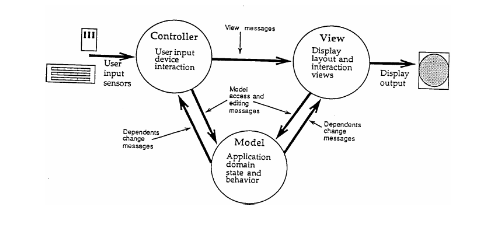
\includegraphics[scale=0.5]{images/TechnicalDesign/MVC.png}
\caption{The Model-View-Controller paradigm}
\label{fig:modelviewcontroller}
\end{center}
\end{figure}

%xxx Make this a graphic, not a photographic image of a graphic 
\begin{figure}[htbp]
\begin{center}
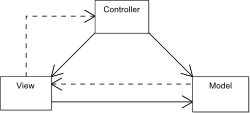
\includegraphics[scale=0.5]{images/TechnicalDesign/ModelViewControllerDiagram.png}
\caption{The Model-View-Controller paradigm AGAIN!}
\label{fig:modelviewcontroller2}
\end{center}
\end{figure}

A global overview of the system architecture can be seen in 
figure~(\ref{fig:globalarchitecture}).
%xxx Make this a graphic, not a photographic image of a graphic 
\begin{figure}[htbp]
\begin{center}
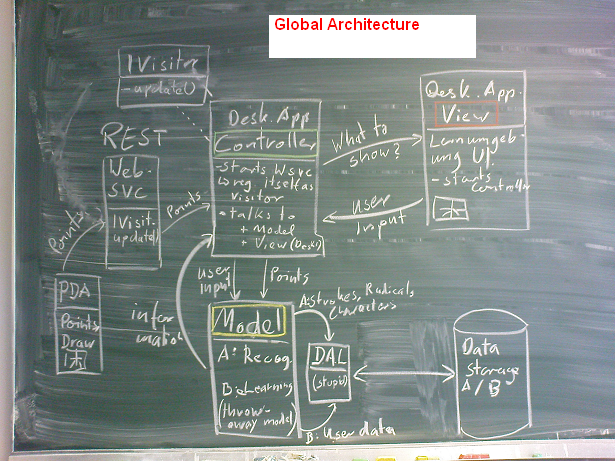
\includegraphics[scale=0.5]{images/TechnicalDesign/GlobalArchitecture.png}
\caption{The global architecture of the software system}
\label{fig:globalarchitecture}
\end{center}
\end{figure}

\subsection{System Data Flow}
\label{sec:arch:systemdataflow}
The system data flow is shown in figure~(\ref{fig:systemdataflow}).
%xxx Make this a graphic, not a photographic image of a graphic 
\begin{figure}[htbp]
\begin{center}
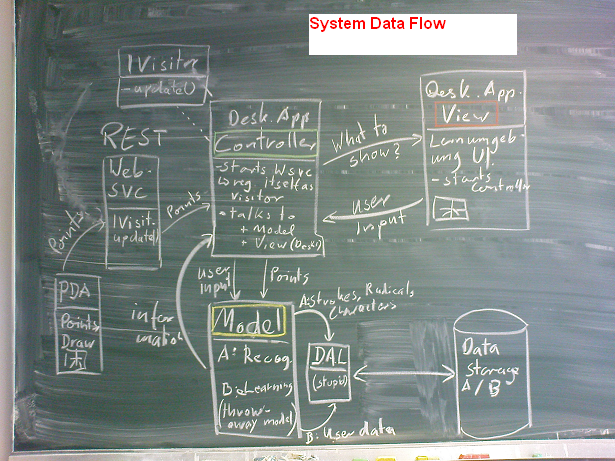
\includegraphics[scale=0.5]{images/TechnicalDesign/SystemDataFlow.png}
\caption{The data flow within the software system}
\label{fig:systemdataflow}
\end{center}
\end{figure}
The controller lies in the centre of the application, it runs on the stationary
device. It contains a web service that is used as an interface to receive data 
from the handwriting input data view. The desktop view is the main interaction 
point for the user. The model contains the logic, while the data access layer 
provides a reusable interface for storing data. The details of 
figure~(\ref{fig:systemdataflow}) are described in subsequent 
sections~\ref{sec:arch:recognitiondataflow} and~\ref{sec:arch:learningdataflow}.

\subsubsection{Communication}
\label{sec:communication} %xxx grep this label, see if it is in use and replace by sec:arch:communication

The communication between the different parts of the application is realised 
in two independet and distinct ways. The communication between the 
modules running under the same process is realised via a messaging system. 
The communication between the modules that run on different devices
or at least as a separate process is realised via a web service.

\emph{Loose coupling} is used here as a term to emphasize that different modules 
in a larger system are only loosely connected and do not depend largely on each 
other. \emph{Coupling} can be understood as the degree of knowledge a module or 
class have of each another. The lesser the knowledge of each other the software 
modules can manage with, the more loose the coupling.

In the course of the design and development cycles of the Kanji Coach, 
it became apparent that it has to be possible to attach different views, 
input devices and data storage systems to the controller. This is due to the 
distributed nature of the application. 
In order to ensure that the handwriting data input view, which currently runs 
on a mobile device, can run on a different device, it had to be loosly coupled 
to the main controller. Therefore, the communication between the handwriting 
input data view and the main controller is realised via a web service. 
Because of this communication structure, it is possible to exchange the 
handwriting data input view with a different one, for instance when running 
the application on a device like a tablet PC. The design of the communication 
structure within the web service is described in greater detail 
in section~\ref{sec:arch:webservice}.

The messaging system that forms the communication structure between the software 
modules running as the same process is realised with a message class that
can be manipulated by the modules using these messages.
Technically, the web service and the controller both run as a subprocess of the 
main desktop view. When the web service receives a request and accompanying data
from the handwriting input data view, both request and data are bundled into an 
encapsulated message and passed to the controller. A similar type of message 
is used for requests from the controller to the model, for instance a recognition
task that needs be performed.

%xxxs. 12 beachten: WICHTIG: selbstgeschriebenens protokoll als alternative
%xxx erwaehnen, ausserdem INKML als datenstruktur
%warum nicht inkml? warum nicht die unipen-struktur?
%selbst mit verwendung von WCF koennte die datenstruktur hilfreich sein.
%ja, aber geschwindigkeit - "get it up there" zaehlt mehr.
%eingabegeraet nimmt ohnehin punktliste vom user,
%umwandlund in irgendein datenformat kann auch spaeter im 
%verarbeitungsprozess erfolgen.


\subsubsection{Recognition Data Flow}
\label{sec:arch:recognitiondataflow}

The recognition data flow is simply the flow of data occuring in a recognition 
scenario. It can be described in \ref{recdataflowDisplayResult} steps
as depicted in figure~(\ref{fig:systemdataflow}).
\begin{enumerate}
  \item \label{recdataflowClear} 
        Clearing the input GUI screen 
        [Controller $\Rightarrow$ Web service $\Rightarrow$ Handwriting data input view]
  \item \label{recdataflowTransmit} 
        Transmitting user input data to the web service 
        [Handwriting data input view $\Rightarrow$ Web service]
  \item \label{recdataflowEncapsulatePass} 
        Encapsulating data into a message and passing 
        it to the controller 
        [Web service $\Rightarrow$ Controller]
  \item \label{recdataflowRequestRecognition} 
        Requesting recognition 
        [Controller $\Rightarrow$ Model] 
  \item \label{recdataflowReturnResult} 
        Returning recognition result 
        [Model $\Rightarrow$ Controller] 
  \item \label{recdataflowDisplayResult} %this should be the last label, otherwise seek for the place where it is used as a number and change it to the new last label there
        Displaying recognition result 
        [Controller $\Rightarrow$ Desktop view]
\end{enumerate}
When the desktop application requests the use to input a Kanji 
character, it sends a message to the web service advising the handwriting data 
input view to clear the screen (step~\ref{recdataflowClear}). 
The handwriting data input view receives the information by polling the web 
service. 
When the user starts drawing on the surface of the handwriting data input view, 
the data is caputered and transmitted to the web service 
(step~\ref{recdataflowTransmit}).
Each stroke is captured and sent individually in order to ensure a faster 
recognition. That way, the recognition process is initiated before the
user finishes writing a character. The web service receives the data and 
creates an encapsulated message. That message is passed to the 
controller (step~\ref{recdataflowEncapsulatePass}).
The controller initiates a request to the model, containing all strokes
subsequent to the last clear screen 
event (step~\ref{recdataflowRequestRecognition}).
The model performs the recognition of the set of strokes and returns the result
or partial result to the controller (step~\ref{recdataflowReturnResult}).
The controller advises the desktop view to display the resulting character
(step~\ref{recdataflowDisplayResult}).

\subsubsection{Learning Data Flow}
\label{sec:arch:learningdataflow}

The learning data flow is the data flow between the learning module of the 
application, the recognition process and the user interaction.
The learning data flow design can be summed up 
in~\ref{learningdataflowDisplayLearningState} steps.
\begin{enumerate}
  \item \label{learningdataflowAskForDrawing} 
        In learning mode or test mode: Asking user to draw a character,
        based on the current lesson data. The controller sends a display
        request to the desktop view.
        [Controller $\Rightarrow$ Desktop view]
  \item \label{learningdataflowRequestStoring} 
        After recognition process: Request storing recognised character in 
        learning profile.
        [Controller $\Rightarrow$ Model]
  \item \label{learningdataflowStoring} 
        Calculation of error points for a character (creation of new data) and
        storage.
        [Model $\Rightarrow$ Data access layer]
  \item \label{learningdataflowReturningLearningState} 
        Returning learning state of character 
        [Model $\Rightarrow$ Controller] 
  \item \label{learningdataflowDisplayLearningState} %this should be the last label, otherwise seek for the place where it is used as a number and change it to the new last label there
        Displaying learning state 
        [Controller $\Rightarrow$ Desktop view
\end{enumerate}
The learning data flow is described in the middle of a user interaction with the
learning application as it illustrates a typical data flow most appropriately
as shown in figure~(\ref{fig:systemdataflow}).

In step~\ref{learningdataflowAskForDrawing} of the learning data flow, the 
controller sends a message to the desktop view with a request to display an 
invitation to the user to draw a specific character.
That step is a part of the general messaging system design that manages the 
communication between the controller and the other modules.
When the recognition process is finished, the character needs to be stored.
The controller requests the model to store the 
character (step~\ref{learningdataflowRequestStoring}).
The logic layer then creates new data, namely the error points of a 
character that naturally become a part of the data flow.
Both the character recognition result and the error points are stored
using the data access layer (step~\ref{learningdataflowStoring}). 
The resulting learning state defines which character will be displayed next.
This calculation result is transmitted from the model to the 
controller after storage in the penultimate 
step~(\ref{learningdataflowReturningLearningState}).
The last step in the learning data flow is the display of the resulting learning 
state to the user in the desktop 
view (step~\ref{learningdataflowDisplayLearningState}).

\subsection{Software Modules}
\label{sec:arch:softwaremodules}

\subsubsection{Handwriting Data Input View}
\label{sec:arch:handwritingdatainputview}

%Put a gfx with a screen shot here.
%http://kleineurl.de/1kfec2.htm
%http://kleineurl.de/1kfeav.htm
%http://kleineurl.de/1kfebg.htm
%http://kleineurl.de/1kfebt.htm
%http://kleineurl.de/1kfecf.htm
%http://kleineurl.de/1kfecs.htm

The handwriting data input view is a graphical user interface. It is designed for
simplicity and usability. It's main task is data capturing.
It contains only an input area, with a cross in order for the user to better 
locate the strokes of the character. This follows a common practice in Kanji 
teaching - a cross departs the writing area in four areas.

There is no \emph{commit} or \emph{finish} button on the handwriting data 
input GUI, since the end of a stroke sequence is handled with a time out in 
the learning module. When the user needs too long to input a character there 
is a problem and help should be offered.
Therefore, it is sufficient to only display a reset button on the writing area.
Whenever the reset button is pressed, the controller is notified of that event.
The current drawing will be removed from the screen. The next user input will
be treated as a new character

In the background of the handwriting data input view the user input is sent to 
the controller module. Besides that, a polling mechanism ensures that any 
messages from the controller to the handwriting input data view are received.
Whenever the user finishes a stroke, the module sends a message via a web service
(see section~\ref{sec:arch:webservice}) to the controller.

\subsubsection{Main View}
\label{sec:arch:mainview}

%xxx graphic of UI design here, maybe a sketch and maybe a screenshot.
The main view of the system is a graphical user interface. It contains a simple
learning environment, a display area for the characters that have been drawn
in the handwriting input area an information area that displays addidional 
information about a character. In a configuration area the user can choose 
between the different lessons the system offers and between a training mode
and a test mode.

\subsubsection{Web Service}
\label{sec:arch:webservice}

%xxx just for the record: see page 50 in booklet to see if this section needs anything else

The main communication module between the handwriting data input view and the 
controller is a web service that runs on the main part of the application
as a subprocess of the controller. When the desktop application requests the 
user to input a Kanji character, it sends a message to the web service 
advising the handwriting data input view to clear the screen. 
The handwriting data input view receives the information by polling the 
web service. However, the main task of the web service is to receive data 
from the handwriting input data view and forward that data to the controller
of the system. 

A web service is a standard means of interoperation between different software
systems, possibly running on different platforms and frameworks. The web service
as such is an abstract definition of an interface, it must be implemented by a 
concrete agent. This agent is a software that sends and receives 
messages~\shortcite{W3C2004}.
The web service in the Kanji Coach system is not a web service in the strict 
sense as intended by the~\shortciteANP{W3C2004}~\citeyear{W3C2004}. It does not 
provide a service as such. The calling client does not receive a reply to a 
request, just an acknoledge message stating that the data has been received. 
A reply with more information is not necessary, since the handwriting data 
input view does not display any information to the user. 
In summary, the web service design for the Kanji Coach system is a web service
in the technical sense, but not in the conceptual sense, as there is no real
crosswise interaction between server and client.
The concrete implementation of the web service is realised with the
\emph{Windows Communication Foundation} (WCF)~\shortcite{Smith2007}.
The WCF uses a \emph{SOAP protocol} (originally: 
\emph{Simple Object Access Protocol}) internally, but the functionality can be 
accessed from within the .NET framework, the concrete SOAP XML messages will 
be created and unpacked into instances of \emph{Common Language Runtime} (CLR) 
objects automatically by the WCF 
framework~\shortcite{W3C1997,Kennedy2001,Smith2007}.

\subsubsection{Recognition Module}
\label{sec:arch:recognitionmodule}
As a part of the model within the MVC paradigm the recognition module plays
a crucial role. From an abstract viewpoint it functions as a black box.
A set of pen trajectories is passed to to the recogniser and a set of
characters is returned as a result, sorted by their matching value.
Additionally, an intended character can be passed to the recognition engine,
such that the recognising module can generate an error analysis based on the 
intended character. If no intended character is given, the recogniser is designed
to use the best result as a basis for an error analysis, with lower confidence
values attached. The detailed design and implementation choices of the 
handwriting recognition engine are described in 
chapter~\ref{chap:handwritingrecognitionengine}.

\subsubsection{Learning Module}
\label{sec:arch:learningmodule}

The learning module is designed as a basic module, mainly for the purpose of 
demonstration. It performs user and character administration tasks.
Each user has a personalised character set, containing the lessons that have been
studied and the error points of each character.
The application is therefore not a vocabulary teaching application, 
but rather a Kanji teaching application. The error point system is rather simple,
the more error points a character has, the more often it will be repeated.
Similarly, the character repetition depends on a vocabulary training method,
that is employed in a systematic fashion. For details see 
section~\ref{sec:concept:characterrepetition}.

\section{Framework and Devices}
\label{sec:frameworkanddevices}

In this section the choices for framework and devices are reviewed briefly.
The decision of which framework to use depends on the operating system.

\subsection{Operating System}
\label{sec:operatingsystem}

Despite the quasi-religious views of which operating system (OS) to use, 
the choice for the Kanji Coach system was simply user oriented. 
The user group 'students of Japanese' consists mainly of non-technical people. 
They usually use a version of the MS Windows operating system. Therefore, even 
when attempting to provide for cross-plattform usability, 
the windows platform is chosen as the basis for the implementation. 
Neither the author nor the application seek to convince anyone of using one 
or the other operating system, therefore it is a logical choice to provide 
software for a system that most people use.

\subsection{Framework}
\label{sec:framework}

The framework to run the system had to fulfill a few criteria.
\begin{itemize}

  \item It should provide an easy-to-use graphical user interface.

  \item It should mirror the natural look-and-feel of the operating system 
        it runs on.

  \item It should be cross-plattform if possible and not be bound to native
        OS-specific code.

  \item It should provide cross-device communication.

  \item It should provide a modern high-level programming language

\end{itemize}

Even though native code that runs directly on the operating system may 
provide for speed and natural look-and-feel, any efforts to port the system
to a different platform become laborious tasks. That rules out the choice of
\emph{C++}.
Generally, the design ideas and framework criteria seem to apply well to both 
the Java platform and the .NET framework. Both provide functionality for an 
easy-to-use GUI. .NET does not mirror the natural look-and-feel of the windows
operating system, it \emph{is} the natural look-and-feel on Windows.
Java has the ability to adopt the look-and-feel of different systems it runs on,
MS Windows as well. The Java virtual machine has long been known to run on 
different platforms, most importantly Linux and Windows, 
while the .NET framework has been implemented for X-Systems by Novell and is 
called \emph{Mono}.
The two differences that gave the .NET framework a slight advantage over Java 
was the comfort and ease the Windows Communication Foundation offers.
The web service functions can be called exactly the way as if they were methods 
of a local software module. The integration of the different parts of the system,
namely the handwriting data input view and the controller does not require much
additional effort. Another advantage of the .NET framework is the programming
language \emph{C\#} that combines many features of the Java with some of C++.
Additionally, C\# offers a smoother handling of generic lists, which is useful
when dealing with lists of mouse coordinates, lists of strokes that are lists
of mouse coordinates and ultimately lists of characters.
With the CLR, which is an ECMA standard like C\#, it is also possible to easily 
integrate with other languages available for the .NET environment.
Lastly, despite the ease of integration with a .NET client, the WCF also allows 
for other systems to connect to a webservice. Since it uses SOAP internally, 
it is possible to communicate with a WCF web service even without .NET, using
so called \emph{POX} (Plain Old XML) messages that can be generated in any
programming language on any framework and operating system.

\subsection{Desktop Computer}
\label{sec:desktopcomputer}

The choice for a stationary computing device is driven by the kind of user
the learning application is aimed at. A notebook computer the way it can be 
bought in any computer store is the closest match to what a user of the system  
most probably will be running. 
The learning system is a standard desktop application with a standard 
MS Windows forms GUI. Therefore, this kind of system is most suitable for the
designed system.
Nevertheless, it is possible to run both the handwriting data input view and
the desktop application on the same PC - for example a tablet PC.
The integration could stay exactly the same.

\subsection{Pen Input Device}
\label{sec:peninputdevice}

The pen input device has been chosen to be a \emph{Personal Digital Assistant} 
computer (PDA). The reason for that design choice is simple. At the time of
drawing the user should be able to see what he is drawing on the writing surface.
At the same time the data should be available to the controller in real-time,
i.e. after a pen-up movement.
The main decision had to be made between a graphics tablet and PDA.
The option of mouse input of charaters was ruled out from the beginning,
because the mouse is not a useful device to enter handrwitten characters.
Graphics tablets like a Wacom tablet are cheaper than a PDA, however,
their distribution on the market and therefore among potential users is small.
The solution with a PDA leaves room to exchange the device that runs the input
area with any mobile device that has the ability to connect to a wireless LAN,
e.g. an iPhone.
Another possibility would be pens that write on paper and also transmit data
to a PC. Those, however, either do not perform the transmission in real-time,
or do not come as plain mouse coordinates but bitmaps or can not connect to
custom made software at all, but only to their OEM software.

%xxx hier zum beispiel noch bericht ueber recherche nach graphic-tablets?!
%und deren APIs siehe seite 35